\documentclass{report}
\usepackage[utf8]{inputenc}
\usepackage[colorlinks=true,urlcolor=black]{hyperref}

\usepackage{listings}
\renewcommand{\lstlistingname}{Frammento}

\usepackage{natbib}
\usepackage{graphicx}
\usepackage{caption}
\usepackage{subcaption}
\usepackage[italian]{babel}
\usepackage{array}
\usepackage{float}
\usepackage{color, colortbl}
\usepackage{wrapfig}
\usepackage{emoji}
\usepackage{grffile}
%\usepackage{bera}  % Have a nice mono-spaced font
\usepackage{xcolor}

\makeatletter
\newcommand{\mypm}{\mathbin{\mathpalette\@mypm\relax}}
\newcommand{\@mypm}[2]{\ooalign{%
  \raisebox{.1\height}{$#1+$}\cr
  \smash{\raisebox{-.6\height}{$#1-$}}\cr}}

\colorlet{punct}{red!60!black}
\definecolor{background}{HTML}{EEEEEE}
\definecolor{delim}{RGB}{20,105,176}
\colorlet{numb}{magenta!60!black}

\addtolength{\footnotesep}{1.5mm}
\renewcommand{\thefootnote}{\textbf{\arabic{footnote}}}

\begin{document}
\hypersetup{linkcolor=black}

\graphicspath{ {./Images/} }

\begin{titlepage}
    \begin{center}
        \vspace*{1cm}
        
        \Huge
        \textbf{Pervasive Computing \\ Laboratorio di Sistemi Software}
        
        \vspace{0.5cm}
        \LARGE
        Relazione di Progetto
        
        \vspace{1.0cm}
        \textbf{Lorenzo Pagnini - Luca Giorgetti}
        
        \vspace{1.5cm}
        
\includegraphics[width=0.4\textwidth]{logo.png}
        
        \vspace{0.5cm}
        \LARGE
        Anno accademico 2021/2022
    
    \end{center}
\end{titlepage}

\tableofcontents

\chapter{Introduzione}
Il progetto si pone come obbiettivo la realizzazione di un applicativo basato su digital twins contestualizzato in ambito sanitario. L'idea è quella di poter creare un'\textit{anima digitale} (o \textit{digital twin}) di dispositivi fisici (detti anche \textit{phisical asset}), utilizzati da medici e infermieri durante gli interventi in sala operatoria. Successivamente, il digital twin permette di realizzare una sua rappresentazione digitale grazie all'utilizzo della realtà aumentata. Uno scenario tipico è quello di poter creare un ologramma di un monitor a parametri vitali che ogni membro del team può visualizzare nella spazio. Quello che si viene a creare è una connessione dell'\textit{asset} con il suo oggetto 3D così che ogni modifica, da parte dell'uomo, porti ad un aggiornamento delle informazioni in entrambi le direzioni. Grazie all'utilizzo di appositi occhiali (\textit{Hololens}, \textit{Magic leap}), ogni infermiere potrà vedere l'ologramma associato ad uno specifico \textit{asset}, in maniera indipendente dal posizionamento di quello fisico e da tutti i suoi colleghi. Ovviamente i dati visualizzati nei dispositivi fisici saranno aggiornati in \textit{real time} anche nell'ologramma.\newline \newline Le tecnologie utilizzate saranno quindi legate all'implementazione dei digital twins, dei rispettivi assets fisici (che in questo caso verranno simulati) e alla sua rappresentazione digitale nella spazio (mixed reality) che permette appunto l'interazione con l'uomo.

\definecolor{Gray}{gray}{0.9}

\chapter{Analisi del dominio}
Questo capitolo verte su tutta l'analisi impiegata sulla conoscenza del dominio dell'applicativo, sull'identificazione dei requisiti, dei casi d'uso nonché sull'analisi dei principi della filosofia Domain Driven Design. \newline \newline Questa fase è stata di grande importanza poiché ci ha permesso, da una parte di avere un ottima conoscenza del dominio applicativo e dall'altra di discutere sui principali aspetti di sviluppo agevolando notevolmente la successiva fase di implementazione.

\section{Il dominio}
In questa sezione verrà descritto il dominio dell'applicativo: verrà presentato l'obiettivo da raggiungere, lo stato dell'arte e l'\textit{ubiquitous language} individuato.
 
\subsection{Obiettivo}

L'obiettivo del progetto è la creazione di un sistema che consenta a tutto il team della sala operatoria (medici, infermieri e anestesisti) di accedere in maniera agevole a tutte le informazioni del paziente durante un intervento chirurgico. In particolare quello che si richiede è di poter digitalizzare attraverso un ologramma il monitor a parametri vitali del paziente. In questo modo, durante un intervento, ogni membro del team può visualizzare il proprio ologramma controllando i relativi valori dei parametri del monitor indipendentemente dalla locazione del dispositivo fisico. \newline \newline Questo approccio porta a semplificare tutte una serie di operazioni che possono essere svolte sul paziente durante l'operazione. Si pensi se durante un intervento è necessario eseguire una TAC d'urgenza: significherebbe trasportare il paziente, tutti i sensori a cui è collegato e il relativo monitor in una stanza adiacente a quella chirurgica con il rischio di perdere del tempo prezioso per problemi che possono incorrere durante il trasferimento. Se si adottasse la soluzione proposta, sarebbe necessario spostare solamente il paziente e non i dispositivi fisici poiché ogni membro del team continua a visualizzare l'ologramma minimizzando il tempo impiegato nel trasferimento del paziente.
Un altro vantaggio è dato dalla connessione in remoto allo stato del monitor del paziente da parte di altri medici che possono essere coinvolti nell'operazione.

\subsection{Stato dell'arte}
Molte grandi città del mondo stanno già impiegando questa tecnologia in ambito sanitario. Ad esempio nell'ospedale di Singapore, i chirurgi utilizzano questo approccio per visualizzare ologrammi di referti dei pazienti, come una risonanza magnetica, durante un intervento chirurgico (maggiori informazioni a questo \href{https://govinsider.asia/citizen-centric/how-a-singapore-hospital-uses-holograms-to-assist-surgery-nuhs-ngiam-kee-yuan/}{link}). Si tratta di un caso simile al nostro ma non del tutto identico. 
La differenza è dovuta al contenuto dell'ologramma cioè quale oggetto tridimensionale si vuole riprodurre nello spazio: nel nostro caso si tratta di un monitor a parametri viali.

\begin{wrapfigure}{l}{0.4\textwidth}
    \centering
    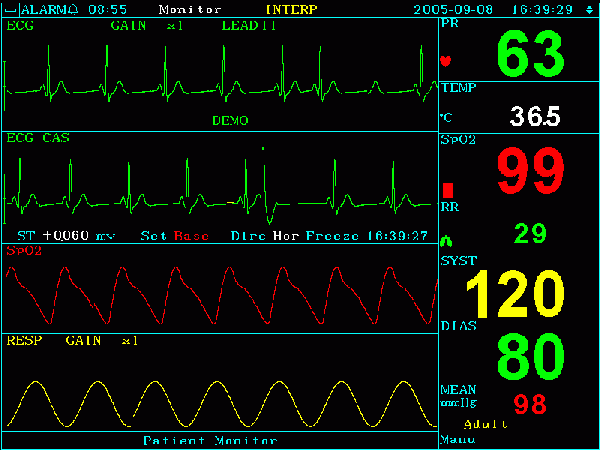
\includegraphics[width=0.4\textwidth]{monitor.png}
\end{wrapfigure}

Durante l'intervento, al paziente vengono collegati diversi sensori per monitorare i parametri vitali.
I valori dei parametri vengono mostrati nel monitor ognuno con uno specifico colore. In particolare per ogni parametro viene mostrato il valore puntuale, l'unità di misura e per alcuni di loro anche un grafico. 
A sinistra è presente un esempio di monitor a parametri vitali ed è quello a cui noi ci siamo basati per la parte di simulazione. I parametri vitali monitorati sono: temperatura, pressione sanguigna, frequenza respiratoria, frequenza cardiaca e saturazione. Per ognuno di questi si è deciso anche di aggiungere un allarme che si attiva qualora il relativo valore supera una certa soglia sia inferiormente che superiormente.

\subsection{Ubiquitous Language}
L'\textit{ubiquitous language} è un dizionario comune di termini usati nella definizione del dominio al fine di eliminare incertezze, imprecisioni e fraintendimenti che possono derivare da ogni membro del team di progetto, esperti del dominio e altri partecipanti. Tale linguaggio è sempre in continuo aggiornamento anche durante tutta la fase di sviluppo e non definito solamente all'inizio. \newline \newline Di seguito è illustrato l'\textit{ubiquitous language} per il nostro applicativo in base al contesto in cui viene utilizzato. Sono presenti tre tabelle: nella tabella \ref{tab:phisical-asset-ubiquitous-language-table} è riportato  l'\textit{ubiquitous language} di termini legati all'asset fisico, la tabella \ref{tab:general-ubiquitous-language-table} descrive termini di carattere generale mentre l'ultima tabella \ref{tab:mixed-reality-ubiquitous-language-table} riporta l'\textit{ubiquitous language} relativo alla realtà aumentata.

\bgroup
\def\arraystretch{1.5}
\begin{table}[H]
    \begin{tabular}{ |m{3cm}|m{3cm}|m{5cm}| } 
        \hline
        \textbf{Termine} & \textbf{Equivalenza} & \textbf{Descrizione}
        \\\hline
        Monitor a parametri vitali & Vital Signs Monitor & Monitor utilizzato per visualizzare i parametri vitali di un paziente durante un intervento chirurgico.
        \\\hline
        Dispositivi fisici &  Phisical Asset & Si intende il monitor a parametri vitali e i relativi sensori.
        \\\hline
        Temperatura & Temperture & Parametro vitale riferito alla temperatura corporea del paziente che è possibile visualizzare nel monitor.
        \\\hline
        Saturazione & Saturation & Parametro vitale riferito alla saturazione del paziente che è possibile visualizzare nel monitor.
        \\\hline
        Pressione sanguigna & Blood Pressure & Parametro vitale riferito alla pressione sanguigna del paziente che è possibile visualizzare nel monitor.
        \\\hline
        Frequenza cardiaca & Heart Frequency & Parametro vitale riferito alla frequenza cardiaca  del paziente che è possibile visualizzare nel monitor.
        \\\hline
        Frequenza respiratoria & Breath Frequency  & Parametro vitale riferito alla frequenza respiratoria del paziente che è possibile visualizzare nel monitor.
        \\\hline
        Allarme &  Alert & Soglia d'allerta di un parametro vitale quando il suo valore è troppo alto o troppo basso rispetto ad uno specifico range.
        \\\hline
        Unità di misura & Unit of measure & Unità di misura utilizzata per rappresentare il valore di uno specifico parametro vitale.
        \\\hline
    \end{tabular}
    \caption{\label{tab:phisical-asset-ubiquitous-language-table}Ubiquitous language utilizzato per descrivere l'asset fisico.}
\end{table}
\egroup

\bgroup
\def\arraystretch{1.5}
\begin{table}[H]
    \begin{tabular}{ |m{2.5cm}|m{2.5cm}|m{7cm}| } 
        \hline
        \textbf{Termine} & \textbf{Equivalenza} & \textbf{Descrizione}
        \\\hline
        Paziente & Patient & Persona che usufruisce del sistema realizzato.
        \\\hline
        Stato del Paziente & Patient Status & L'insieme delle informazioni relative ai parametri vitali del paziente durante un intervento.
        \\\hline
        Cartella Clinica & Medical Record & Documento che raccoglie le informazioni di tipo medico-anagrafico del paziente. 
        \\\hline
        Team & Team & L'insieme delle persone che utilizzeranno il sistema realizzato ovvero tutti i soggetti attivi nella sala operatoria durante un intervento chirurgico.
        \\\hline
    \end{tabular}
    \caption{\label{tab:general-ubiquitous-language-table}Ubiquitous language utilizzato per termini di carattere generale.}
\end{table}
\egroup

\bgroup
\def\arraystretch{1.5}
\begin{table}[H]
    \begin{tabular}{ |m{2.5cm}|m{2.5cm}|m{7cm}|} 
        \hline
        \textbf{Termine} & \textbf{Equivalenza} & \textbf{Descrizione}
        \\\hline
        Ologramma & Hologram  & Rappresentazione tridimensionale del monitor a parametri vitali nello spazio.
        \\\hline
    \end{tabular}
    \caption{\label{tab:mixed-reality-ubiquitous-language-table}Ubiquitous language utilizzato per la realtà aumentata.}
\end{table}
\egroup


\section{Requisiti}
Una delle fasi fondamentali dell’intero processo di analisi, è ricaduta nella definizione dei requisiti che il progetto dovrà soddisfare. Questi verranno raffinati in corso d’opera andando a creare una comprensione del dominio sempre più approfondita. Verranno descritti i requisiti di business, utente, funzionali e non funzionali.

\subsection{Business}
I requisiti di business sono così descritti:

\begin{itemize}
    \item Il prodotto dovrà fornire un monitoraggio a distanza. Questo consentirà al personale incaricato di poter controllare i parametri vitali del paziente in remoto;
    
    \item Il prodotto dovrà consentire di agevolare l'insieme delle operazioni svolte in sala operatoria che richiedono lo spostamento di dispositivi fisici.
\end{itemize}

\subsection{Utente}
I requisiti utente sono così descritti:

\begin{itemize}
    \item Il prodotto deve permettere di creare la cartella clinica del paziente quando questo viene ricoverato in ospedale;
    
    \item Il paziente deve poter essere identificato univocamente tramite il suo codice fiscale;

    \item L'ologramma deve avere un interfaccia intuitiva simile il più possibile a quella di un monitor a parametri vitali fisico, con possibilità di un menù per poter fare un focus su uno specifico parametro vitale;
    
    \item L'ologramma deve avere un sistema di allerta se i valori dei parametri vitali sono al di sopra o al di sotto di uno specifico range;
    
    \item Il prodotto deve poter fornire la possibilità di personalizzare i parametri vitali. In particolare il personale incaricato potrà personalizzare il range di ogni parametro vitale e l'unità di misura con cui quel dato è rappresentato;
    
    \item I dati mostrati nell'ologramma devono essere aggiornati in tempo reale, minimizzando il tempo di latenza;
    
    \item L'accesso dello stato del paziente in sala operatoria tramite l'ologramma deve essere fatto per mezzo di un QR code;

    \item La comunicazione dello stato di un paziente tra il monitor a parametri vitali fisico e l'ologramma deve essere fatto per mezzo di un QR code.
    
    \item L'ologramma dovrà mostrare la cartella clinica del paziente.
\end{itemize}

\subsection{Funzionali}
Si elencano i requisiti funzionali per ognuno dei seguenti contesti:

\begin{itemize}
    \item Accesso del paziente in ospedale;
    \item Intervento chirurgico.
\end{itemize}

L'immagine \ref{pic:use-cases} mostra i caso d'uso del sistema relativi ai contesti citati.

\begin{figure}[ht]
    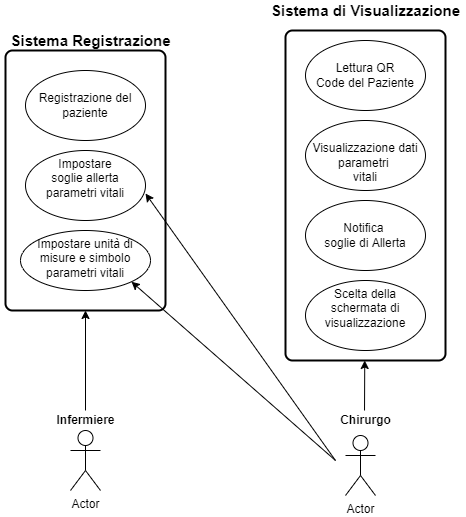
\includegraphics[width=11cm]{casiUso.png}
    \centering
    \caption{\label{pic:use-cases}Casi d'uso del sistema.}
\end{figure}

\subsubsection{Accesso del paziente in ospedale}
Quando il paziente deve essere ricoverato in ospedale è necessario registrarlo nel sistema informatico dell'ospedale. L'operatore incaricato dovrà quindi creare la sua cartella clinica compilando i dati richiesti. Successivamente, il chirurgo se lo ritiene necessario può configurare le soglie di allerta per i parametri vitali e infine verrà generato il relativo QR code che sarà utilizzato per il riconoscimento del paziente in sala operatoria.

\subsubsection{Intervento chirurgico}
Se è necessario eseguire un operazione chirurgica al paziente, il chirurgo può utilizzare oltre al monitor a parametri vitali fisico anche quello virtuale grazie alla visualizzazione di un ologramma. Per fare ciò sarà necessario scannerizzare il QR code del paziente (generato in fase di ricovero) sia nel monitor fisico sia nell'ologramma al fine di creare la connessione tra i due sistemi per la ricezione dei dati. In questo modo il chirurgo potrà visualizzare nell'ologramma i dati relativi ai parametri vitali del paziente, eventuali allarmi, i grafici, i valori puntuali e scegliere di monitorare un preciso parametro anziché avere una schermata generale di tutti. Inoltre sarà possibile visualizzare la cartella clinica del paziente compilata in fase di ricovero.

\subsection{Non funzionali}
I requisiti non funzionali sono così descritti.

\subsubsection{Usabilità}
l sistema deve fornire agli utenti finali un’interfaccia chiara, semplice, ben organizzata in modo da poter utilizzare al meglio tutte le sue funzionalità messe a disposizione e visualizzate.

\subsubsection{Legati al Sistema}
\begin{itemize}
    \item \textbf{Reattività}. L'utente non deve percepire ritardi tra la visualizzazione dei dati nel monitor a parametri vitali fisico e la visualizzazione degli stessi nell'ologramma;
    
    \item \textbf{Fault tolerance}. Deve essere implementato un adeguato sistema di gestione degli errori affinché le interruzioni involontarie non compromettono la salute del paziente durante un intervento chirurgico;
    
    \item \textbf{Sicurezza}. Utilizzando \textit{Azure Digital Twins} i dati salvati nel cloud e quelli in transito tra due o più componenti di Azure sono crittografati;
    
    \item \textbf{Scalabilità}. L’applicativo deve necessariamente consentire di aumentare o diminuire il numero di pazienti gestiti senza influire negativamente sulla prestazione del sistema. 
\end{itemize}

\subsection{Implementativi}
Il software dovrà essere realizzato utilizzando la filosofia \textit{Domain Driven Design}. Dovranno inoltre essere utilizzate metodologie di DevOps al fine di automatizzare e integrare quanti più processi possibili. Si utilizzerà il servizio Azure Digital Twins (PaaS - Platform As A Service) per la gestione dei digital twins e l'interfacciamento con i diversi clients. Per la parte di mixed reality si utilizzerà Unity e i visori Microsoft Hololens.

\section{Aspetti di Domain Driven Design}

\subsection{Core-Domain}
\subsection{Sub-Domain}
\subsection{Bounded Context}
\subsection{Context Map}

\chapter{Processo di Sviluppo}

\section{Gestione di Progetto}
Si è utilizzato \textit{Git} per effettuare il versioning del codice durante lo sviluppo attraverso la piattaforma GitHub.
L’utilizzo che ne abbiamo fatto è descritto nella figura \ref{pic:workflow}: il branch di default è sempre il \textit{main}, al quale \textit{development} è sempre allineato. Ogni volta che era necessario implementare una nuova \textit{feature} veniva creato un brach da \textit{development}. Nel caso in cui debbano essere prodotti degli hotfix o risolti dei bug, essi vengono svolti su un branch che parte da \textit{development} e vi ritorna, prima di essere mergiato nuovamente su \textit{main}.

\begin{figure}[ht]
    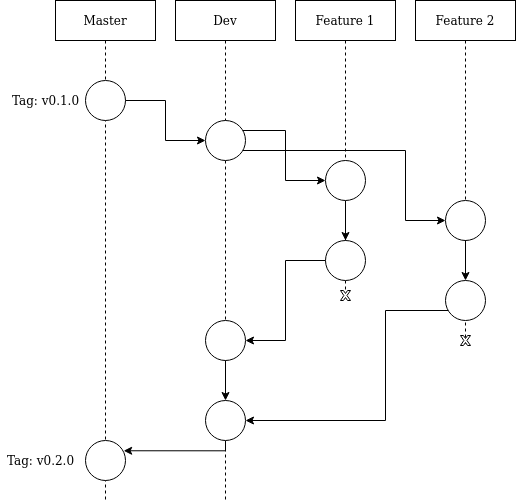
\includegraphics[width=8cm]{git-workflow.png}
    \centering
    \caption{\label{pic:workflow}Workflow del progetto.}
\end{figure}

 Successivamente, a lavoro ultimato, veniva creata una pull request per mergiare sul branch \textit{development} e infine sul \textit{main}.

\subsection{Versioning}
\subsection{Licensing}

\section{Build Automation}
La build automation è stata realizzata utilizzando il servizio delle GitHub Actions. Tutti i \textit{job} implementati venivano eseguiti sul branch \textit{development} ad ogni commit e pull-request. Inoltre i singoli \textit{job} specifici di una particolare \textit{features} venivano eseguiti anche sul branch di implementazione di quella \textit{features}. Vengono descritti tutti i \textit{job} realizzati:

\begin{itemize}
    \item \textbf{build-and-deploy-app-function}: utilizzato per deployare le \textit{azure function} in azure;
    
    \item \textbf{build-simulator}: utilizzato per eseguire la build del simulatore e creare il rispettivo \textit{artifact};
    
    \item \textbf{build-client}: utilizzato per eseguire la build del clien (lato simulatore) e creare il rispettivo \textit{artifact};
    
    \item \textbf{compile-report}: utilizzato per compilare la relazione in Latex e creare il relativo file \texttt{.pdf};
    
    \item \textbf{release}: utilizato per creare le releae del simulatore e client;
    
\end{itemize}

Inoltre sono stati implementati ulteriori due \textit{job} con lo scopo di notificarci se la build automation è terminata con successo o con un fallimento. La notifica si basa nel inviare un messaggio su un bot Telegram realizzato appositamente per il progetto (accessibile tramite questo \href{https://telegram.me/AzureHealthcareNotificator_bot}{\textit{link}}). Questi \textit{job} sono stati utilizzati nei branch \textit{development} e \textit{report}.  
\begin{itemize}
    \item \textbf{jobs-failure}: notifica tramite un messaggio sul bot Telegram che la build è fallita;  
    
    \item \textbf{jobs-success}: notifica tramite un messaggio sul bot Telegram che la build è completata con successo;  
\end{itemize}

\section{Continuos Integration}

\chapter{Design Architetturale}
\label{chap:architectural-design}
In questo capitolo verrà descritta l'architettura del sistema, illustrando i componenti principali. Si rimanda al capitolo \ref{chap:detailed-design} per ulteriori informazioni riguardante il codice dell'applicativo e le specifiche di implementazione.

\section{Architettura}

\subsection{Generale}

Considerando l'obiettivo del progetto abbiamo deciso di modellare la rappresentazione virtuale della nostra entità fisica (monitor a parametri vitali) attraverso i digital twins. Questo modello permette infatti di essere alimentato in maniera continua dai dati provenienti da sensori, realizzando un'\textit{anima digitale} del monitor. Questo concetto è impiegato maggiormente in ambiti industriali, permettendo di effettuare analisi all'interno dei processi produttivi. Anche in ambito \textit{healthcare}, questo modello offre dei vantaggi: nel nostro caso, il digital twin è stato utilizzato per:

\begin{itemize}
    \item \textbf{Concettualizzazione}: permette di ottenere un'efficace rappresentazione virtuale, anche real-time con l'impiego della mixed reality per la visualizzazione;

    \item \textbf{Collaborazione}: concettualizzazione del monitor in modo che possa essere condivisa da più persone, anche in remoto.
\end{itemize}

Dopo aver modellato i dati, ci siamo preoccupati di scegliere dove posizionare i digital twin. Le opzioni tra cui scegliere sono tre: 

\begin{itemize}
    \item \textbf{Edge}: i digital twin vengono deployati all'interno dell'asset fisico;
    
    \item \textbf{Cloud}: i digital twin vengono deployati su una piattaforma cloud;
    
    \item \textbf{Fog}: i digital twin vengono deployati all'interno di una rete locale (LAN).
\end{itemize}

La nostra scelta è ricaduta sul cloud poiché abbiamo previsto lo scenario in cui la virtualizzazione può essere acceduta anche al di fuori dell'ospedale in cui viene eseguita l'operazione. Questa motivazione ci ha fatto escludere la tipologia fog. 

\subsection{Dettaglio}
L'architettura generale del sistema è illustrata nella figura \ref{pic:architecture}.

\begin{figure}[ht]
    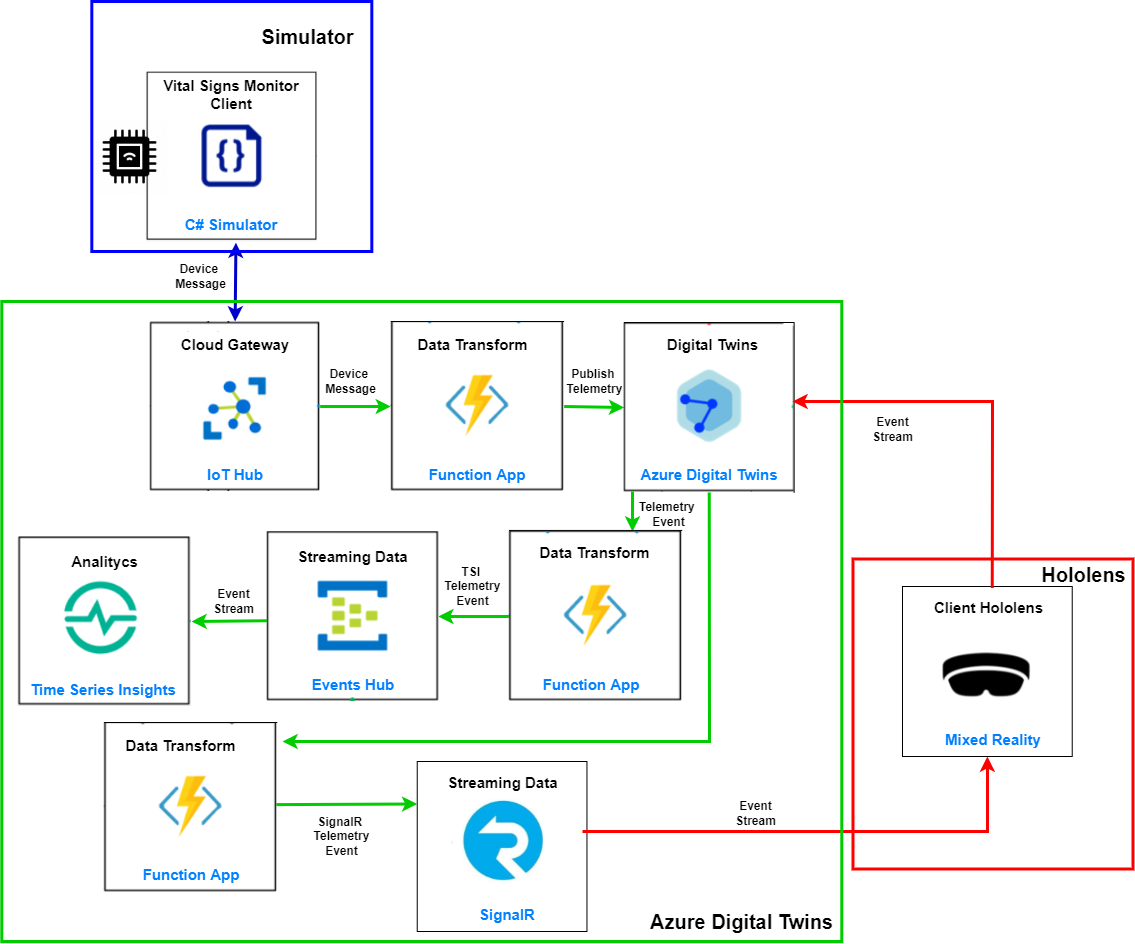
\includegraphics[width=10.3cm]{architecture.png}
    \centering
    \caption{\label{pic:architecture}Architettura del sistema.}
\end{figure}

Le componenti principali dell'architettura sono:

\begin{itemize}
    \item \textbf{Healthcare Vital Signs Monitor}: emula il monitor a parametri vitali fisico. Invia i dati ad Azure Digital Twins. Nella figura \ref{pic:architecture} è la componente blu;
    
    \item \textbf{Azure Digital Twins (ADT)}: una piattaforma PaaS fornita da Microsoft che mette a disposizione un'insieme di funzionalità per poter implementare e gestire i Digital Twins. Questa piattaforma permette di creare un gemello digitale dell'asset fisico, memorizzare un'insieme di dati che costituiscono lo stato del digital twin e propagarlo ad altri clients: in questo caso Hololens. Nella figura \ref{pic:architecture} è la componente verde;
    
    \item \textbf{Healthcare Hololens Client}: riceve lo stato dell'asset fisico da Azure Digital Twins tramite web socket. Invia i dati di configurazione dell'ologramma ad Azure Digital Twins. Nella figura \ref{pic:architecture} è la componente rossa;  
\end{itemize}

\subsection{Protocolli di comunicazione}

Per l'integrazione dei componenti della nostra architettura abbiamo dovuto scegliere alcuni protocolli di comunicazione. \newline \newline Per la comunicazione tra Healthcare Vital Signs Monitor e Azure Digital Twins abbiamo utilizzato il protocollo \textit{https} mentre per la comunicazione tra Azure Digital Twins e Healthcare Hololens Client la scelta è ricaduta sulla web socket. Questo protocollo crea un canale bidirezionale tra client e server, consentendo una comunicazione a bassa latenza. Inoltre, supporta l'utilizzo di un browser web permettendoci in futuro di sviluppare un applicazione web per la visualizzazione dei dati real-time. Queste motivazioni ci hanno fatto propendere per l'utilizzo di una web socket piuttosto che l'utilizzo del protocollo MQTT, molto diffuso in ambito IoT.

\section{Healthcare Vital Signs Monitor}
Questa componente permette di creare la cartella clinica di un paziente compilando uno specifico form. Una volta completata viene creato il dispositivo IoT nell'IoT Hub e vengono creati i due digital twins in ADT: quello relativo al paziente e quello relativo al monitor a parametri vitali. A questo punto si è in grado eseguire il simulatore su uno specifico paziente. I parametri vitali monitorati dal simulatore sono cinque:

\begin{itemize}
    \item Temperatura corporea (colore bianco) misurata in gradi Celcius (°C);
    \item Frequenza cardiaca (colore verde) misurata in BPM (Beat per minute);
    \item Frequenza respiratoria (colore verde) misurata in RPM (Revolution per minute);
    \item Saturazione (colore rosso) misurata in percentuale (\%);
    \item Pressione sanguigna (di colore gialla) misurata in millimetri di mercurio o Torr (mmHg).
\end{itemize}

\begin{figure}[ht]
    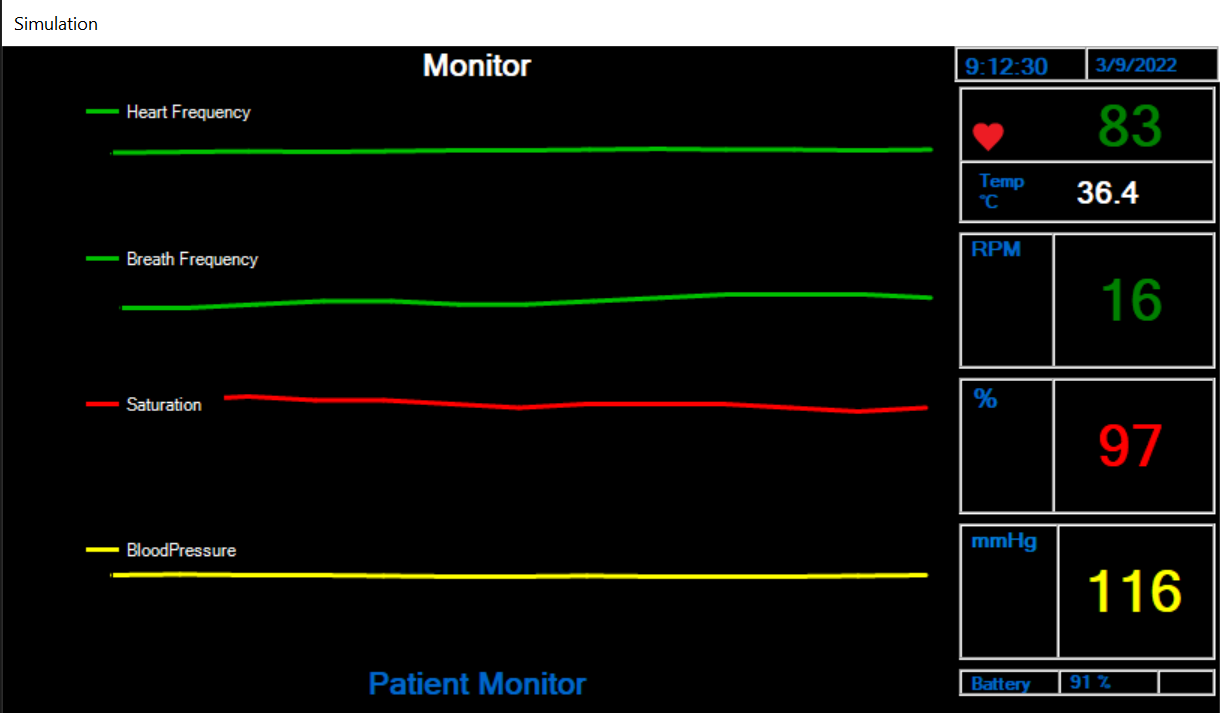
\includegraphics[width=11cm]{simulator.png}
    \centering
    \caption{\label{pic:simulator}Simulatore.}
\end{figure}

Come si evince dalla figura \ref{pic:simulator}, per tutti questi parametri vitali (eccetto la temperatura), è mostrato un grafico degli ultimi N campioni acquisiti con il colore di riferimento. \newline \newline Per tutti i parametri è presente anche un sensore di allerta che si attiva se un valore supera (o diventa inferiore) il valore massimo (o minimo) di un determinato range (specifico per ogni parametro vitale). Tali sensori sono posti a sinistra dei grafici e alla destra del valore della temperatura e della batteria. Se si prende in considerazione l'immagine \ref{pic:simulator}, questi non sono visibili poiché tutti i valori sono nella norma. L'infermiere o il chirurgo possono personalizzare i range e l'unità di misura. \newline \newline A destra del simulatore invece possiamo individuare due colonne: la prima indica l'unità di misura usata per rappresentare il valore del parametro vitale mentre la seconda mostra il suo valore numerico. In alto a destra si trova la data e l'orario corrente mentre in basso a destra il livello della batteria rimanente.
\newline \newline Una volta che il simulatore è in esecuzione, ogni volta che ha nuovi dati, questi vengono trasmessi al ADT.

\section{Azure Digital Twins}
Questa è la componente più corposa del sistema che funge da server. I diversi componenti vengono descritti a seconda dell'ordine di esecuzione in accordo con l'immagine \ref{pic:architecture}:

\begin{itemize}

    \item \textbf{IoT Hub}: è l'Hub di Azure che offre un back-end per ospitare sul cloud e connettere qualsiasi dispositivo IoT. All'interno dell'Hub sono presenti i dispositivi IoT ``\textit{virtuali}" relativi a monitors a parametri vitali di specifici pazienti. Tali dispositivi vengono aggiunti nell'Hub quando viene compilata la cartella clinica di un nuovo paziente. Tali dispositivi ricevono i dati dal simulatore e li propagano all'istanza \textit{Azure Digital Twins} attraverso l'esecuzione di una \textit{azure function};
    
    \item \textbf{Azure function}: è un servizio cloud che fornisce l'infrastruttura e le risorse necessarie per eseguire le applicazioni. L'azure function in questione è chiamata \textit{ProcessHubToDTEvents}. Tale funzione è in grado di eseguire il parsing del contenuto del messaggio inviato dal simulatore e aggiornare le proprietà dei digital twins.
    
    \item \textbf{Azure Digital Twins}: rappresenta l'istanza dove risiedono i digital twins. Per ogni paziente creato esistono due digital twins: quello del paziente e quello del monitor a parametri vitali. Essi sono legati da una relazione ``\textit{un paziente ha un monitor associato}". Tramite questa istanza è possibile consultare lo stato delle proprietà dei digital twins e fare queries. Ogni qualvolta che i digital twins vengono aggiornati vengono eseguite in parallelo due azure function descritte nel punto successivo;
    
    \item \textbf{Azure functions}. La prima azure function è chiamata \textit{ProcessDTUpdatetoTSI} ed è dedicata a propagare lo stato dei digital twins al Time Series Insights (TSI). La seconda azure function è chiamata \textit{SignalRFunction} ed implementa la libreria SignalR per poter comunicare con il client Hololens. Tale funzione ha due sotto-funzioni: la prima (\textit{negotiate}) permette di creare la connessione con il client, la seconda (\textit{broadcast}) permette di inviare i dati al client;
    
    \item \textbf{Time Series Insights (TSI)}: è una soluzione per archiviare, visualizzare ed eseguire queries su grandi quantità di dati relativi a quelli generati dai dispositivi IoT. Nel nostro applicativo i dati vengono solamente archiviati. Una funzionalità futura potrebbe essere quella di eseguire delle queries a partire dai clients per mostrare uno storico dei dati prodotti dal simulatore;
    
    \item \textbf{SignalR}: SignalR è una libreria sviluppata da Microsoft che implementa una web socket e permette al server di inviare notifiche asincrone alle applicazioni clients creando una connessione bi-direzionale. Risulta essere performante per applicazioni \textit{real-time} come nel nostro caso.
\end{itemize}

\section{Healthcare Hololens Client}
L'ultima componente del nostro sistema è il client Hololens che permette di usare la mixed reality. Dopo aver indossato gli occhiali e avviata l'applicazione, è necessario scansionare il QR code del paziente. Quando il QR code viene riconosciuto viene mostrato l'ologramma del monitor a parametri vitali e la cartella clinica del paziente. Una volta avviato il simulatore, l'ologramma del monitor si popolerà di nuovi dati e aggiornerà i valori dei parametri. Per avere un maggior controllo sulla visualizzazione dei dati abbiamo pensato ad un menù interattivo con cui scegliere quale tipo di dato osservare: se visualizzare la situazione generale del paziente o focalizzarsi su un singolo parametro vitale. Grazie alla mixed reality, il grande vantaggio è dato dall'interazione dell'uomo con l'ologramma. Infatti è possibile spostare il monitor ovunque si voglia nello spazio reale, ``\textit{prendendolo}" appunto con le mani. Per cambiare schermata, invece è possibile premere su uno dei pulsanti del menù interattivo. Per una maggiore comodità abbiamo pensato fosse utile far si che gli ologrammi si spostino automaticamente in base a dove l'uomo si sta muovendo o guardando nell'ambiente (ad esempio come la funzionalità \textit{follow me}). Per fare ciò, è possibile attivare il pulsante PIN \emoji{pushpin} premendolo (in alto a destra di ogni ologramma). Come impostazione predefinita, tale pulsante è disattivato: in questo modo gli ologrammi rimangono fermi nell'ambiente se non vengono spostati direttamente dall'uomo.

\subsection{QR Code}
La parte relativa alla lettura del QR Code non ha nessuna interfaccia di interesse. Una volta avviata l'app su Hololens verrà mostrato un \textit{loading progress} in attesa della lettura di un QR Code. Dopo aver mostrato il QR Code, se è valido, verrà mostrato il menù, il monitor a parametri vitali e la scheda del paziente. \newline \newline Per l'implementazione di questa parte ci siamo avvalsi del seguente \href{https://github.com/LocalJoost/QRCodeService}{\textit{repository}}.

\subsection{Menù Interattivo}
Il menù si presenta come nell'immagine \ref{pic:menu-hololens}. E' composto da sette pulsanti:
\begin{itemize}
    \item il pulsante \textit{Home} permette di visualizzare il monitor a parametri vitali di un paziente come quello mostrato nel simulatore;
    
    \item ogni pulsante, in riferimento ad un parametro vitale, permette di visualizzare il suo pannello dedicato;
    
    \item il pulsante \textit{Values} permette di visualizzare solamente i valori dei parametri vitali del paziente, senza mostrare grafici;
    
    \item il pulsante \textit{Exit} permette di uscire dal programma.
\end{itemize}

\begin{figure}[ht]
    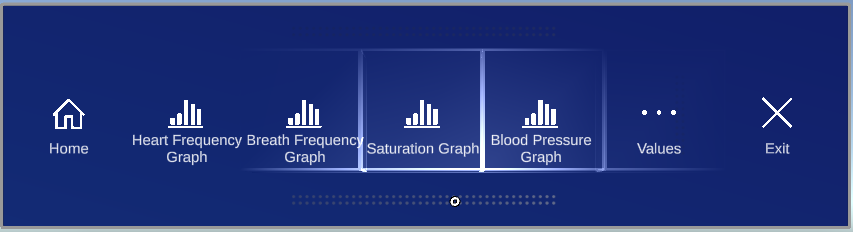
\includegraphics[width=11cm]{hololensMenu.PNG}
    \centering
    \caption{\label{pic:menu-hololens}Menu di Hololens.}
\end{figure}

\subsection{Monitor a parametri vitali}
L'immagine \ref{pic:example-hololens} mostra alcuni esempi: nella figura \ref{pic:monitor-hololens} è mostrato il monitor a parametri vitali generale mentre  nell'immagine \ref{pic:saturation-hololens} è presente il pannello dedicato ad un singolo parametro vitale. In questo caso si è scelto la saturazione premendo il pulsante \textit{Saturation Graph} dal menù. Durante la realizzazione dei pannelli della mixed reality si è cercato di preservare il più possibile la grafica del simulatore così da evitare confusione tra i due monitors: quello fisico e quello virtuale. \newline \newline Come descritto in precedenza, l'immagine \ref{pic:monitor-hololens} mostra a sinistra i sensori di allerta dei parametri vitali: di colore bianco quando i valori sono nella norma e di colore rosso quando assumono valori di pericolo per il paziente. Nell'esempio, la temperatura e la frequenza cardiaca sono in una situazione critica e vengono caratterizzati da un sensore di allarme di colore rosso. Proseguendo verso destra sono presenti i grafici dei quattro parametri vitali più importanti.
\begin{figure}
     \centering
     \begin{subfigure}[b]{0.8\textwidth}
         \centering
         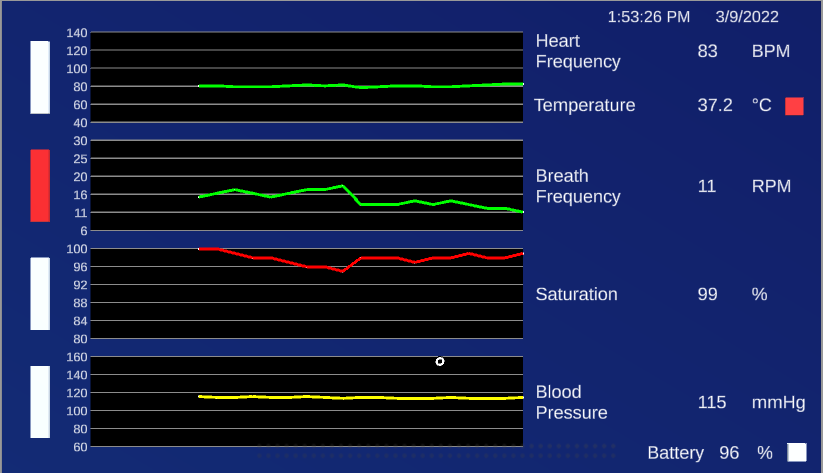
\includegraphics[width=\textwidth]{hololensMonitor.PNG}
         \caption{Monitor a parametri vitali generale.}
         \label{pic:monitor-hololens}
     \end{subfigure}
     \hfill
     \begin{subfigure}[b]{0.8\textwidth}
         \centering
         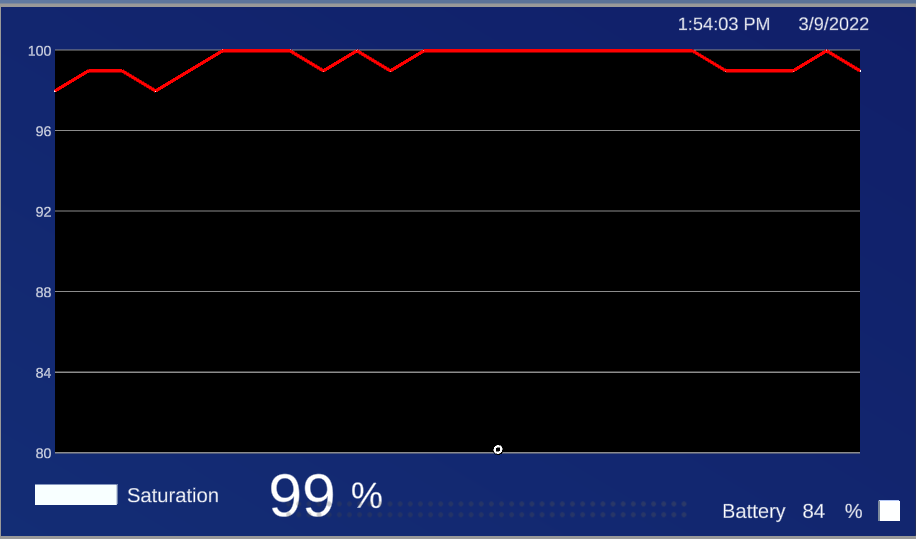
\includegraphics[width=\textwidth]{SaturationHololens.PNG}
         \caption{Monitor della saturazione.}
         \label{pic:saturation-hololens}
     \end{subfigure}
     \hfill
        \caption{Esempi di monitor a parametri vitali in Hololens.}
        \label{pic:example-hololens}
\end{figure}
Successivamente sono presenti tre colonne e contengono rispettivamente il nome del parametro vitale, il valore numerico e l'unità di misura utilizzata. \newline \newline La figura \ref{pic:saturation-hololens} mostra il pannello focalizzandosi su uno specifico parametro vitale. In questo modo si può osservare con più accuratezza e livello di dettaglio l'andamento del grafico. Tutti gli altri valori sono mostrati sotto il grafico.

\subsection{Pannello del Paziente}
L'ultimo ologramma è quello legato al paziente e mostra la sua cartella clinica. Tale pannello contiene le seguenti informazioni:
\begin{itemize}
    \item il nome e il cognome;
    \item il sesso;
    \item l'età, il peso e l'altezza
    \item l'indice di massa corporea;
    \item una descrizione riguardante la sua situazione clinica prima di entrare in sala operatoria. Può contenere note del team, il suo stato di salute e tutto ciò che è rilevante e da tenere in considerazione quando si effettua l'operazione;
    \item il suo codice fiscale;
\end{itemize}

Questo pannello contiene informazioni statiche poiché durante l'intervento queste non possono essere modificate. Il pannello del paziente si presenta come è mostrato nella figura \ref{pic:patient-panel}.

\begin{figure}[ht]
    \includegraphics[width=9.5cm]{PatientPanel.PNG}
    \centering
    \caption{\label{pic:patient-panel}Esempio del pannello del paziente.}
\end{figure}

\chapter{Design di Dettaglio}
 \label{chap:detailed-design}
In questo capitolo verrà illustrata l'organizzazione del codice per i componenti dell'architettura, i pattern utilizzati e le principali scelte implementative.

\section{Organizzazione del Codice}

Il progetto è consultabile al seguente \href{https://github.com/lucagiorgettismp/AzureHealthcareDigitalTwins}{\textit{repository}} di GitHub. Il repository è organizzato nelle seguenti directory:

\begin{itemize}

    \item \textbf{VitalSignsMonitorSimulator}: contiene la soluzione C\# del simulatore;
    
    \item \textbf{DTDLModels}: contiene i modelli \texttt{.json} per la definizione dei digital twins;
    
    \item \textbf{AzureTools}: contiene la soluzione C\# di tutte le azure function implementate;

    \item \textbf{HololensClient}: contiene il progetto Unity per la parte di mixed reality;
        
    \item \textbf{doc}: contiene la documentazione in formato \texttt{.latex} e \texttt{.pdf}.
\end{itemize}

\subsection{Simulatore}
Il simulatore è un progetto .NET scritto in C\# che contiene tre moduli:
\begin{itemize}
    \item \textbf{Client}:
    \item \textbf{Simulator}:
    \item \textbf{Common}: 
\end{itemize}

\subsection{Azure Digital Twins}

\subsubsection{Modelli}

\subsubsection{Azure function}

\subsection{Mixed Reality - Hololens}

\section{Pattern utilizzati}

\chapter{Deployment}
Il progetto sviluppato si compone di tre applicazioni:

\begin{itemize}
    \item Applicazione Client backend;
    \item Applicazione Simulator;
    \item Applicazione Hololens.
\end{itemize}

Le prime due sono rilasciate su GitHub, pertanto basterà recuperare l'ultima release dal nostro repository a questo \href{https://github.com/lucagiorgettismp/AzureHealthcareDigitalTwins/releases}{\textit{link}}.
Allegati alla release si trovano i file .zip contenenti gli eseguibili di Client e Simulator.

\section{Client backend}
L'applicazione client di backend permette di visualizzare le schede paziente precedentemente create e la creazione di nuovi pazienti. Per poter utilizzare il sistema progettato, è necessario che almeno un paziente sia stato creato prima di avviare il simulatore, in quanto al momento della creazione della scheda paziente viene creato anche il device IoTHub per il relativo monitor parametri vitali.

\begin{figure}[H]
    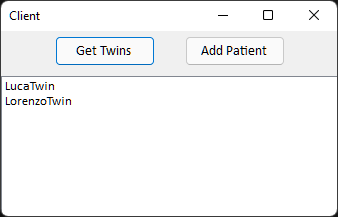
\includegraphics[width=6cm]{client_screen.png}
    \centering
    \caption{\label{pic:client-deployment}Schermata principale del client.}
\end{figure}

\section{Simulatore backend}
Questa applicazione permette di simulare l'asset fisico, pertanto è necessario che venga avviata per emettere dati sul monitor parametri vitali del paziente. \newline \newline All'apertura, viene recuperata la lista dei devices presenti, e una volta selezionato quello desiderato (eventualmente creato tramite il Client al paragrafo precedente), è possibile configurare range dei valori, unità di misura e soglie di allarme. Diversamente, il simulatore viene avviato con i valori di default.
Con il device selezionato, è possibile avviare il monitor parametri vitali che ad ogni iterazione genererà nuovi valori che verranno notificati al digital twin.\\
\newline Se il simulatore è spento, non viene aggiornato il digital twin, pertanto non viene inviato nessun messaggio su SignalR.

\begin{figure}[H]
    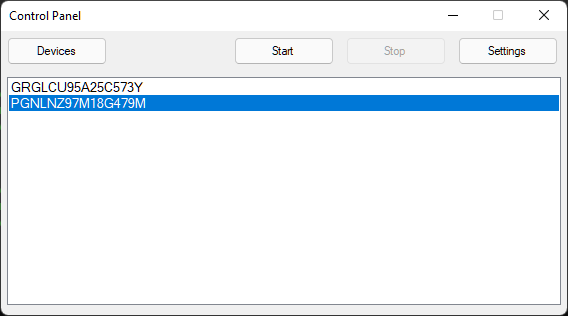
\includegraphics[width=10cm]{simulator_screen.png}
    \centering
    \caption{\label{pic:simulator-deployment}Schermata di selezione device.}
\end{figure}

\section{Applicazione Hololens}
Non essendo rilasciata su Microsoft Store, la nostra applicazione deve essere prima compilata, ed in seguito rilasciata sul device Hololens.

Durante lo sviluppo abbiamo utilizzato Unity v2020.3.4f1 e Visual Studio 2019 v16.11.11.

\subsection{Import di Mixed Reality Toolkit}
Prima di aprire il progetto, è necessario importare le componenti del Mixed Reality Toolkit.
\begin{enumerate}
    \item Avviare il Mixed Reality Toolkit (MixedRealityFeatureTool) scaricato
precedentemente.
    \item Fare clic sull’icona dell’ingranaggio.
    \item  Nella sezione Feature Settings, attivare “Show preview releases” e cliccare su OK.
    \item Fare clic su Start.
    \item Impostare il percorso del progetto Unity creato precedentemente e fare clic su “Discover Features”.
    \item Nella sezione “Mixed Reality Toolkit” selezionare “Mixed Reality Toolkit foundation”
    \item Nella sezione “Platform Support” selezionare “Mixed Reality OpenXR Plugin”.
    \item Cliccare su ”Get Features”.
    \item Cliccare su “Validate”, poi su OK e infine su Import.
    \item Cliccare su “Approve” e poi su “Exit”, a questo punto i componenti dovrebbero essere stati importati in Unity correttamente.
\end{enumerate}

\subsection{Configurazione di Mixed Reality Toolkit}
Aprendo il progetto su Unity dovrebbe comparire la finestra “MRTK Project Configurator”. In caso contrario, la si può aprire da menù \\ 
Mixed Reality > Toolkit > Utilities > Configure Project for MRTK.
\begin{enumerate}
    \item Controllare che tutte le opzioni siano spuntate e cliccare su “Apply”, a questo punto Unity dovrebbe riavviarsi.
    \item Selezionare Edit > Project Settings.
    \item Selezionare XR Plug-in Management > Install XR Plug-in Management.
    \item In Universal Windows Platform attivare “ XR Plug-in Management > Install XR Plug-in Management”, “OpenXR” e “Microsoft HoloLens feature set”.
    \item Se sono presenti dei warning cliccare sul punto esclamativo e poi su “Fix All”, dovrebbero scomparire.
\end{enumerate}

\subsection{NuGet}
E' necessario installare NuGet in Unity e scaricare i pacchetti utilizzati dal nostro progetto:

\begin{enumerate}
    \item Installare NuGet il wiki presente al seguente link: \url{https://github.com/GlitchEnzo/NuGetForUnity}.
    \item Riavviare Unity.
    \item Scaricare i pacchetti utilizzati tramite menu NuGet > Restore Packages.
\end{enumerate}

\subsection{Build e Deploy}

\begin{enumerate}
    \item In Unity selezionare File > Build Settings.
    \item Cliccare su Add Open Scenes per aggiungere le scene.
    \item Configuare la build come mosttrato in figura \ref{pic:build-settings}.
    
    \begin{figure}[H]
        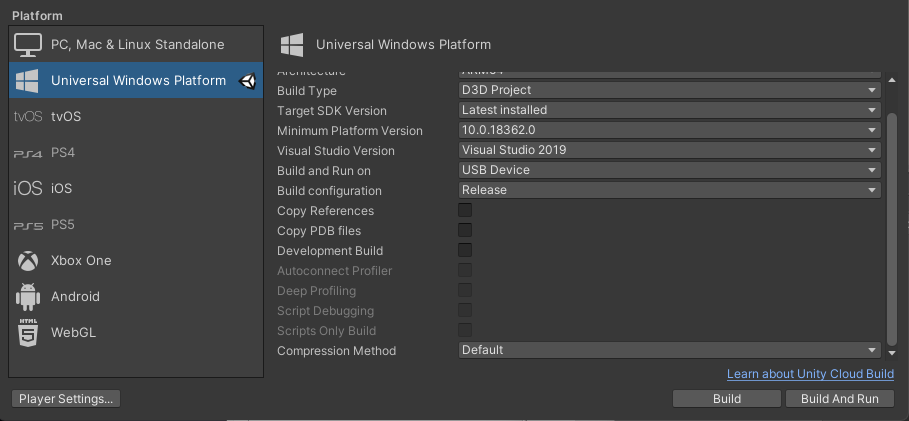
\includegraphics[width=12cm]{Images/hololens_build_settings.png}
        \centering
        \caption{\label{pic:build-settings}Build settings.}
    \end{figure}
    
    \item Cliccare su “Build” e selezionare la cartella delle build (solitamente “Builds”, nella directory del progetto Unity)
    \item Dopo aver compilato dovrebbe aprire una nuova finestra del gestore dei file, entrare nella cartella delle build e avviare il progetto di Visual Studio.
    \item In Visual Studio selezionare “Release”, architettura: “ARM64”, target: “Device” 
    \item Collegare Hololens 2 al PC (Usare le porte USB della scheda madre se possibile)
    \item Quando si fa il deploy da un nuovo PC per la prima volta bisogna fare il pairing dei device:
    \item Su Visual Studio avviare il deploy da Build > Deploy solution, verrà richiesto un PIN.
    \item Su Hololens andare in Settings > For Developers e cliccare su “Pair”, comparirà un PIN, inserirlo in Visual Studio.
    \item A questo punto si può accedere all’app installata direttamente dal menu delle applicazioni di Hololens 2.
\end{enumerate}

\subsection{Creazione QR code}
    E' possibile utilizzare uno dei QR code presenti in all'interno della release su GitHub, oppure generarne uno custom; in questo caso:
    \begin{enumerate}
        \item Andare all'url \url{https://www.qrcode-monkey.com/en/#text}.
        \item Inserire una stringa di tipo Json fatta come segue:
        \begin{lstlisting}[language=json, firstnumber=1]
{"deviceId": "CODICE_FISCALE_DEL_PAZIENTE"}
        \end{lstlisting}
        \item Generare e scaricare il QR code appena creato.
    \end{enumerate}

Una volta avviata l'applicazione su Hololens, inquadrare il QR code. \\
\newline Quando viene rilevato l'identificativo del paziente, verranno caricate le informazioni sul paziente, il menù di selezione delle schermate e la schermata precedentemente selezionata (o di default la schermata Home se si tratta della prima apertura).

\chapter{Conclusione}

Al termine dell'elaborato, possiamo ritenerci più che soddisfatti del risultato ottenuto, essendo riusciti a raggiungere gli obiettivi prefigurati.\newline

L'utilizzo delle tante tecnologie, non conosciute o viste in maniera superficiale all'inizio del lavoro (\textit{Unity}, \textit{Hololens} e \textit{Azure}), è stato sicuramente il primo scoglio da superare, ed effettivamente, da una parte ha rallentato la tabella di marcia ma allo stesso tempo ci ha permesso di acquisire nuove conoscenze. Queste potranno rivelarsi utili in futuro, vista che si tratta di tecnologie e piattaforme sempre più studiate ed utilizzate.\newline

Inizialmente avevamo fatto un'indagine per lo sviluppo dei digital twins su \textit{Eclipse Ditto} e \textit{Hono}, tentativo che non ha portato a nulla di concreto per via del malfunzionamento del sevizio di test online e dell'elevato utilizzo delle risorse per farlo eseguire sulle nostre macchine. Il problema ci ha fatto apprezzare quanto il migrare ad una soluzione come \textit{Azure}, di tipo PaaS (Platform as a Service) abbia semplificato la configurazione dei servizi e lo sviluppo su di essi.
\newline

A causa dell'inesperienza con le tecnologie utilizzate, con il senno di poi avremmo considerato con più attenzione aspetti che avevamo trascurato inizialmente. Ad esempio attribuire sin da subito agli oggetti di \textit{Unity} la giusta dimensione per essere visualizzati correttamente tramite \textit{Hololens}, piuttosto che l'attenzione alle performance della nostra applicazione.\newline

Nel complesso, nonostante le difficoltà, siamo riusciti ad implementare ed integrare tutto quello che avevamo previsto: il simulatore del monitor a parametri vitali, il client per la creazione del paziente, l'infrastruttura \textit{Azure Digital Twins} e tutti gli ologrammi appartenenti alla realtà aumentata. \newline

Uno dei problemi più spinosi è stato il \textit{porting} su piattaforma \textit{Hololens} delle librerie testate ed utilizzate su Windows, cosa che ritenevamo più fluida. Alcune di queste librerie hanno invece dato problemi solamente a \textit{runtime}, rallentando lo sviluppo. 
Inoltre la piattaforma \textit{Unity} si è dimostrata ostica nel riuscire a lavorare con più macchine sulla stessa scena, per via del modo in cui vengono assegnati gli id degli oggetti, costringendoci a ripetere il binding di questi ad ogni modifica. \newline

In conclusione, siamo certi che la tecnologia dei \textit{Digital Twins} sarà sempre più pervasiva visto il grande potenziale che può offrire: sia in termini di contributo sia sull'ampia scelta di settori in cui può essere utilizzata: dal settore ospedaliero a quello industriale passando per qualsiasi settore ingegneristico, per via degli innumerevoli vantaggi che può portare al netto dei costi di implementazione.

\end{document}